\section{Einleitung}

\section{Team}

\begin{frame}
    \frametitle{\insertsection}
    \vfill
    \begin{columns}
        \begin{column}[c]{0.2\textwidth}
            
\includegraphics[height=3em]{fig/logo_ess}  
        \end{column}
        \begin{column}[c]{0.7\textwidth}
            \textbf{Fachgebiet Elektrische Systeme \& Sensorik}\\
            LG3A, 1. Stock, Siemens-Halske-Ring 14, Cottbus
        \end{column}
    \end{columns}
    
    \vfill

    \begin{columns}[onlytextwidth]
        \begin{column}{0.5\textwidth}
            \textbf{Vorlesung:} Prof. Dr.-Ing. Markus Gardill
            \begin{itemize}
                \item markus.gardill@b-tu.de
                \item Tel.: 0355 69-3410
            \end{itemize}
            \begin{center}
                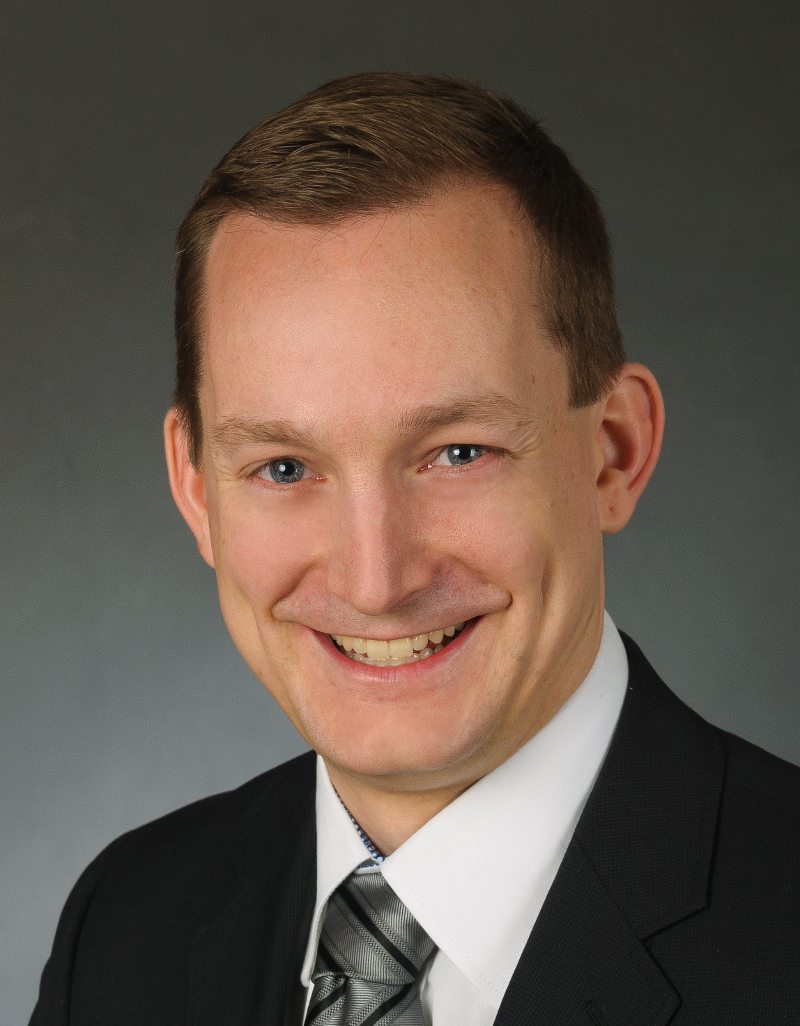
\includegraphics[height=3cm]{fig/photo_gardill}
            \end{center}
        \end{column}
        \begin{column}{0.5\textwidth}
            \textbf{Seminar:} Dipl.-Ing. Marcus Heide
            \begin{itemize}
                \item marcus.heide@b-tu.de
                \item Tel.: 0355 69-3425
            \end{itemize}
            \begin{center}
                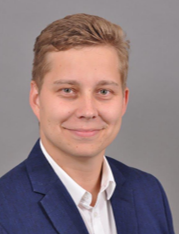
\includegraphics[height=3cm]{fig/photo_heide}
            \end{center}
        \end{column}
    \end{columns}

\end{frame}

\section{Vorlesungsinhalt}

\begin{frame}
    \frametitle{\insertsection}
    \vfill
    \begin{itemize}

        \item Sensor-Charakteristika \emph{[SEC]}
        \item Positionsbestimmung \emph{[POS]}
        \item Geschwindigkeitsmessung \emph{[GES]}
        \item Drehzahlmessung \emph{[DRE]}
        \item Messung mechanischer Beanspruchung und Kraftmessung \emph{[KRA]}
        \item Temperaturmesstechnik \emph{[TEM]}
        \item Inertialsensoren \emph{[IMU]}
        \item Durchflussmesstechnik \emph{[FLO]}
        \item Gassensoren \emph{[GAS]}
        \item Biologische und medizinische Sensoren \emph{[BIO]}
        \item Sensoren für Strahlung und Licht \emph{[RAD]}
        
    \end{itemize}
\end{frame}

\section{Literatur}
\begin{frame}
    \frametitle{\insertsection}
   
    \begin{tabular}{m{0.75\textwidth}m{0.2\textwidth}}
        \parbox{0.7\textwidth}{\textbf{Sensortechnik}\\Hans-Rolf Tränkler, Leonhard Reindl.\\Handbuch für Praxis und Wissenschaf\\Springer-Lehrbuch\\Springer Vieweg Verlag, 2. Auflage, Berlin, Heidelberg 2014\\
        \href{https://link.springer.com/book/10.1007/978-3-642-29942-1}{\underline{DOI 10.1007/978-3-642-29942-1}}\\
        \emph{Tränkler [SEC,POS,GES,DRE,KRA,TEM,FLO,GAS]}} &\includegraphics[height=4cm]{fig/Sensortechnik}\\
    \end{tabular}


    \begin{tabular}{m{0.75\textwidth}m{0.2\textwidth}}
        \parbox{0.7\textwidth}{\textbf{Sensoren in Wissenschaft und Technik}\\Ekbert Hering, Gert Schönfelder\\Funktionsweise und Einsatzgebiete\\Springer Vieweg Verlag, 2. Auflage, Wiesbaden 2018\\
        \href{https://link.springer.com/book/10.1007/978-3-658-12562-2}{\underline{DOI 10.1007/978-3-658-12562-2}}\\
        \emph{Hering [POS,KRA,TEM,FLO,BIO,RAD]}} &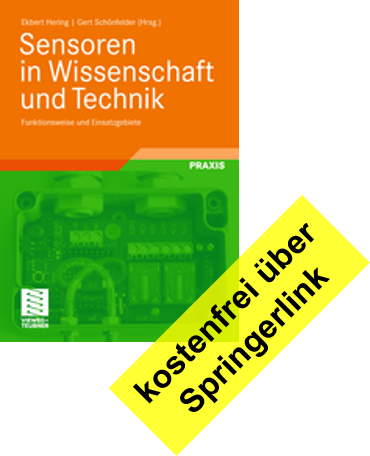
\includegraphics[height=4cm]{fig/sensoren_in_wissenschaft_und_technik}\\
    \end{tabular}

    
\end{frame}

\section{Literatur}
\begin{frame}
    \frametitle{\insertsection}
    \vfill
    \begin{tabular}{m{0.75\textwidth}m{0.2\textwidth}}
        \parbox{0.7\textwidth}{\textbf{Elektrische Messtechnik}\\Elmar Schrüfer, Leonhard Reindl\\Bernhard Zagar\\Messung elektrischer\\und nichtelektrischer Größen\\Carl Hanser Verlag\\12. Auflage, München 2018\\
        \href{https://www.hanser-kundencenter.de/fachbuch/artikel/9783446456549}{\underline{DOI 10.3139/978-3-446-45698-3}}\\
         \emph{Schrüfer [POS,KRA,TEM,FLO]}} &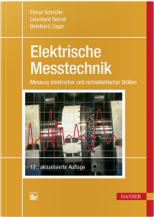
\includegraphics[height=3.5cm]{fig/elektrische_messtechnik}\\
    \end{tabular}

    \vfill

\end{frame}